\documentclass[12pt, titlepage]{article}
\usepackage{indentfirst}
\usepackage[margin=1in]{geometry}
\usepackage{hyperref}
\usepackage{pgfplots}
\usepackage{float}
\usepackage{amsmath}
\usepackage{etex}
\renewcommand\refname{Works Cited}

\title{\normalsize How do FIDE chess ratings compare to USCF chess ratings of the top 10 chess players in the US?}
\date{\normalsize Candidate Number: hyg172 \\ May 2020 \\ Word Count:}

\begin{document}
\maketitle
\tableofcontents
\newpage

\section{Exploration}
\subsection{Introduction}
As a young child, I've always been interested in the idea of quantifying and relating objects using numbers. This was initially a usefool tool in visualizing basic arithmetic. When I started playing tournament chess, I recieved a chess rating, or a number used to quantify one's chess strength relative to others. There are multiple such systems that give chess player ratings, for example online chess websites such as Lichess and Chess.com have their own rating systems, and even countries have their own rating systems. However, the governing body of chess, FIDE, has their own rating system that allows a standard rating for comparison between countries with otherwise different rating systems. This led to the foci of the investigation on how FIDE ratings compare to USCF ratings with respect to the top 10 players in the US and also comparing the strengths of the top 10 players of the top 6 countries.
\subsection{Research Questions}
How do the FIDE ratings compare to USCF ratings of the top 10 chess players in the US?

How different are the ratings between the top 10 players of the top 6 chess country federations?
\subsection{Hypothesis}
I predict that USCF ratings will be not much different from FIDE ratings. However, USCF ratings may be slightly higher as the overall pool of players with FIDE ratings has stronger players.

I predict that there will be a statistically significant difference between the FIDE ratings of the top 10 players of the top 6 countries as they have different concentrations of strong players. 

\section{Analysis}
\subsection{USCF vs FIDE}
\subsubsection{Data}
Suprisingly, the top 10 players by USCF rating differ from FIDE's list of the top 10 US players by FIDE rating. This difference is due to the fact that FIDE and USCF tournaments have different criteria for a tournament to be valid. Due to this, we will find the respective USCF ratings of the top 10 US players by FIDE rating. Nevertheless, the top players American players by FIDE and USCF rating are the same, just in different order.

\begin{figure}[H]
\centering
\begin{tabular}{rr}
FIDE & USCF\\
\hline
2822 & 2894\\
2765 & 2826\\
2758 & 2834\\
2736 & 2836\\
2712 & 2787\\
2683 & 2744\\
2677 & 2758\\
2673 & 2749\\
2660 & 2733\\
2659 & 2748\\
\end{tabular}
    \caption{FIDE vs USCF ratings}
  \end{figure}
  
The USCF top player list and the FIDE list accurate as of December 2019.

\begin{figure}[H]
\centering
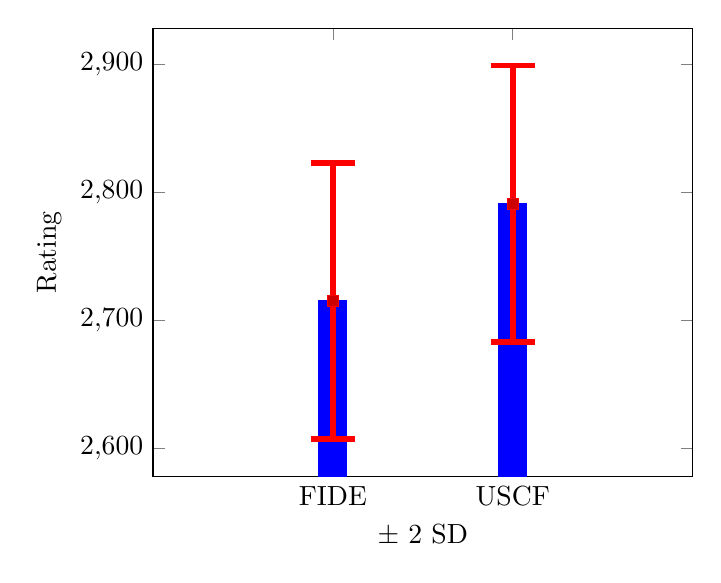
\begin{tikzpicture}
\begin{axis}[
symbolic x coords={FIDE, USCF},
xtick=data,
enlarge x limits = 1,
xlabel = {\(\pm \) 2 SD},
ylabel = {Rating}
]
\addplot+[ybar,fill=blue] coordinates {
(FIDE, 2715)
(USCF, 2791)
};
\addplot+[only marks, error bars/.cd,
y dir=both, y explicit, error bar style={line width=2pt}, error mark options={
rotate=90,
red,
mark size=8pt,
line width=2pt}] 
coordinates {(FIDE, 2715) +-(0,108) (USCF, 2791) +-(0,108)
};
\end{axis}
\end{tikzpicture}
\caption{FIDE and USCF Ratings}
\end{figure}

\begin{figure}[H]
\centering
\begin{tabular}{rr}
Standard Deviation & Mean\\
\hline
54 & 2715\\
\end{tabular}
    \caption{FIDE rating}
\end{figure}

\begin{figure}[H]
  \centering
\begin{tabular}{rr}
Standard Deviation & Mean\\
\hline
54 & 2791\\
\end{tabular}
    \caption{USCF rating}
\end{figure}

\subsubsection{2 Sample T-Test}
Null Hypothesis: There is no significant difference between the mean FIDE rating and the mean USCF rating. FIDE and USCF ratings are indeendent.

Alternate Hypothesis: There is a significant differrence between the mean FIDE rating and the mean USCF rating. FIDE and USCF ratings are indeendent.

Test Statistic: 
\begin{equation*}
\begin{split}
    t_{(n-1)} \; \textrm{d}f & = \dfrac{(\overline{x_{1}} - \overline{x_{2}}) - (\mu_{1} - \mu_{2})}{\sqrt{\dfrac{(s_{1})^{2}}{n_{1}}} + \dfrac{(s_{2})^{2}}{n_{2}}} \\
    & = \dfrac{(2715-2791) - (0)}{\sqrt{\dfrac{(54)^{2}}{10} + \dfrac{(54)^{2}}{10}}} = -3.16
\end{split}
\end{equation*}

p-value: P(t \(\leq\) -3.16) = 0.005

\subsubsection{Data based answer to the research question}
Because the p-value is less than 0.05, the null hypothesis cannot be accepted. Therefore, we provisionally accept the alternate hypothsis that there is a significant difference between USCF and FIDE ratings.

\subsubsection{Linear Regression}
\begin{figure}[H]
\centering
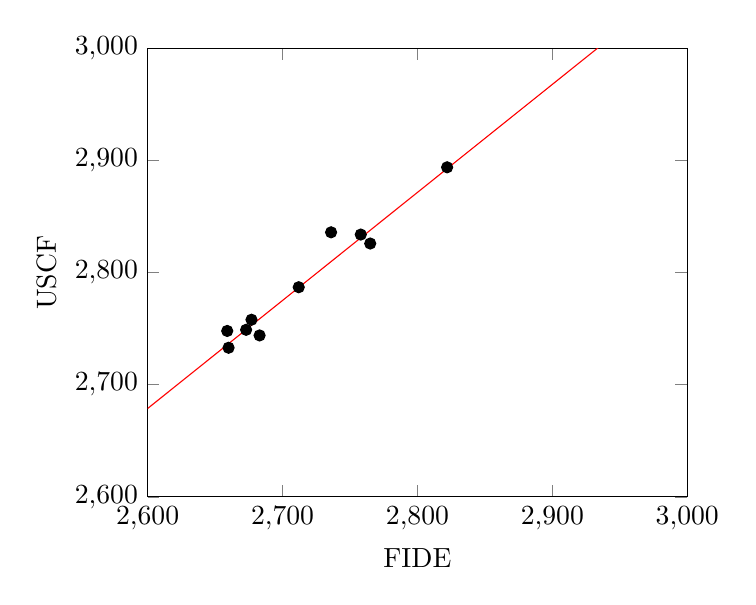
\begin{tikzpicture}
    \begin{axis}[
        xmin = 2600,
        domain = 2600:3000,
        ymin = 2600,
        ymax = 3000,
        xmax = 3000,
        xlabel = FIDE,
        ylabel = USCF
        ]
    \addplot[only marks] coordinates {
    (2822,2894)
    (2765,2826)
    (2758,2834)
    (2736,2836)
    (2712,2787)
    (2683,2744)
    (2677,2758)
    (2673,2749)
    (2660,2733)
    (2659,2748)   
    };
    \addplot+[no marks, color=red]{0.964 * x + 172.391};
    \end{axis}
\end{tikzpicture}
    \caption{USCF vs FIDE rating}
\end{figure}

We will use a linear regression to test how well FIDE and USCF ratings relate to each other among the top 10 US players.

USCF = 0.964 FIDE + 172
The linear regression results in an r value of 0.976 and an \(r^{2}\) value of 0.953. This shows that there is a very strong correlation between USCF and FIDE ratings. This is true despite the fact that the average USCF and FIDE ratings have a statistically significant difference.

\subsection{Comparing Chess Ratings of the Top 6 Countries}
\subsubsection{Data}
\begin{figure}[H]
  \centering
\begin{tabular}{lrrrrrr}
 & Russia & USA & China & India & Ukraine & Armenia\\
\hline
 & 2777 & 2822 & 2805 & 2758 & 2698 & 2773\\
 & 2774 & 2765 & 2758 & 2721 & 2685 & 2689\\
 & 2753 & 2758 & 2732 & 2716 & 2685 & 2663\\
 & 2752 & 2736 & 2726 & 2654 & 2678 & 2642\\
 & 2747 & 2712 & 2705 & 2648 & 2662 & 2641\\
 & 2731 & 2683 & 2683 & 2639 & 2660 & 2641\\
 & 2726 & 2677 & 2669 & 2638 & 2650 & 2632\\
 & 2723 & 2673 & 2667 & 2637 & 2644 & 2617\\
 & 2705 & 2660 & 2664 & 2636 & 2634 & 2613\\
 & 2704 & 2659 & 2640 & 2630 & 2631 & 2611\\
\(\sum\) & 27392 & 27145 & 27049 & 26677 & 26627 & 26522\\
 \(\overline{x}\) & 2739.2 & 2714.5 & 2704.9 & 2667.7 & 2662.7 & 2652.2\\
SD & 25.75 & 54.40 & 50.67 & 45.92 & 23.15 & 48.65\\
\end{tabular}
\caption{Top 6 Countries and their top 10 players}
\end{figure}

This data was retreived from FIDE's Top Chess Federations. It is interesting to see that Russia is the only country with its top 10 players having a rating higher than 2700. Standard Deviation (SD) was calculated using a Ti-84 calculator.

\begin{figure}[H]
\centering
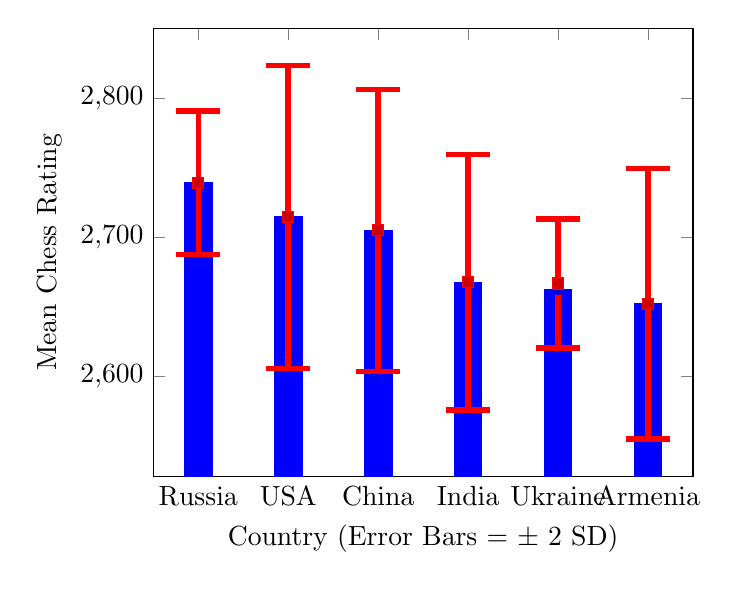
\begin{tikzpicture}
\begin{axis}[
symbolic x coords={Russia, USA, China, India, Ukraine, Armenia},
xtick=data,
xlabel = {Country (Error Bars = \(\pm \) 2 SD)},
ylabel = {Mean Chess Rating}
]
\addplot+[ybar,fill=blue] coordinates {
(Russia, 2739.2)
(USA, 2714.5)
(China, 2704.9)
(India, 2667.7)
(Ukraine, 2662.7)
(Armenia, 2652.2)
};
\addplot+[only marks, error bars/.cd,
y dir=both, y explicit, error bar style={line width=2pt}, error mark options={
rotate=90,
red,
mark size=8pt,
line width=2pt}] 
coordinates {(Russia, 2739.2) +-(0,51.5) (USA, 2714.5) +-(0,108.8)(China, 2704.9) +-(0,101.34) (India, 2667.7) +-(0,91.84) (Ukraine, 2666.7) +-(0,46.3) (Armenia, 2652.2) +-(0,97.3) 
};
\end{axis}
\end{tikzpicture}
\caption{Mean Chess Rating by Country}
\end{figure}

\subsubsection{ANOVA Test}
Null Hypothesis: There is not a significant difference in mean ratings among the six countries. 

Alternate Hypothesis: There is a significant difference in mean ratings among the six countries. The observed differences are not due to random sampling variation.

Variation between groups:
\begin{equation*}
\begin{split}
    SST & = [\frac{27392^{2}}{10} + \frac{27145^{2}}{10} + \frac{27049^{2}}{10} + \frac{26677^{2}}{10} + \frac{26627^{2}}{10} + \frac{26522^{2}}{10}] \\ 
    & - [\frac{(27392+27145+27049+26677+26627+26522)^{2}}{60}] \\
    & = 59140.8 
\end{split}
\end{equation*}

Variation within groups:
\begin{equation*}
\begin{split}
    SSE & = [2777^{2} + .. + 2611^{2}] - [\frac{27392^{2}}{10} + \frac{27145^{2}}{10} + \frac{27049^{2}}{10} + \frac{26677^{2}}{10} + \frac{26627^{2}}{10} + \frac{26522^{2}}{10}] \\
    & = 100814.8 
\end{split}
\end{equation*}

Finding the squared standard error would require squaring each of the 60 data points. As the standard square error is easily calculated using a calculator, only first and last terms are shown.
\begin{figure}[H]
\centering
\begin{tabular}{lrlrr}
 & SS & DF & MS & F\\
Treatments & 59140.8 & k-1=6-1=5 & 11828.16 & 6.336\\
Errors & 100814.8 & N-k = 60-6=54 & 1866.94074 & \\
\end{tabular}
\end{figure}

Dividing the sum of the squares by the degress of freedom for both the treatments and the errors results in the mean of the squares. Dividing the mean of the squares of treatments by the mean of the squares of errors results in a Fischer value of approximately 6.336.

Test Statistic: F(5,54) = 6.336

p-value: P(F\(>\)6.336) = 1.0736 x \(10^{-4}\)

\subsubsection{Data based answer to the research question}
The probabilty of the null hypothesis is 1.0736 x \(10^{-4}\). Therefore the data does not support the null hypothesis and we can provisionally accept the alternate hypothesis that there is a significant difference in mean chess ratings among the top six countries.

\section{Conclusion}
As we can see, there is a significant difference in the strength of the top 6 chess countries as shown by the ANOVA test. We also found out that a chess federation's rating system can differ from FIDE's ranking system, as shown by the 2 sample test between FIDE and USCF ratings. 

\subsection{Extensions}
It would be interesting to see whether there is still a significant difference between the top 3 chess country federations. It would also be interesting to look at countries concentration of grandmasters, international masters, as well as titled players as a measure of strength. It would also be interesting to see which country's rating system is most similar to FIDE ratings. Additionally, it would be interesting to see how online ratings compared to FIDE ratings.

% \newpage
% \begin{appendix}
% p\section{Calculating standard deviation using Python}
% \begin{verbatim}
% import statistics

% # Russia
% print(statistics.stdev([2777, 2774, 2753, 2752, 2747, 2731, 2726, 2723, 2705, 2704]))

% # USA
% print(statistics.stdev([2822, 2765, 2758, 2736, 2712, 2683, 2677, 2673, 2660, 2659]))

% # China
% print(statistics.stdev([2805, 2758, 2732, 2726, 2705, 2683, 2669, 2667, 2664, 2640]))

% # India 
% print(statistics.stdev([2758, 2721, 2716, 2654, 2648, 2639, 2638, 2637, 2636, 2630])) 

% # Ukraine
% print(statistics.stdev([2698, 2685, 2685, 2678, 2662, 2660,2650, 2644, 2634, 2631]))

% # Armenia
% print(statistics.stdev([2773, 2689, 2663, 2642, 2641, 2641,2632, 2617, 2613, 2611]))
% \end{verbatim}
% \end{appendix}

\newpage
\begin{thebibliography}{thewidest}
\bibitem{Unsort}
\url{https://ratings.fide.com/top_lists.phtml}

\bibitem{Unsort}
  \url{http://www.uschess.org/component/option,com_top_players/Itemid,371?op=list&month=1912&f=usa&l=R:Top%20Overall.&h=}

\bibitem{Unsort}
\url{Explorable.com (Jun 6, 2009). ANOVA. Retrieved Feb 19, 2020 from Explorable.com: https://explorable.com/anova}

\bibitem{Unsort}
\url{https://ocw.mit.edu/courses/aeronautics-and-astronautics/16-881-robust-system-design-summer-1998/lecture-notes/l7_anova4.pdf}

\bibitem{Unsort}
\url{https://www.itl.nist.gov/div898/handbook/prc/section4/prc433.htm}
\end{thebibliography}
\end{document}








